\chapter{\MakeUppercase{Кинематика конечностей робота}}
\section{Общее положение} \label{sec:kin_general}
Как было сказано ранее, оптимизация распределения масси робота потребовала введения в кинематическую структуру ноги замкнутого контура.
Проблема такой кинематики в механической сложности ее реализации с точки зрения конструктора. Из-за особенностей и требований, описанных в пункте \ref{sec:leg_design}, конструкция ноги получилась, как на рисунке ниже.
\begin{figure}[h]
    \centering
    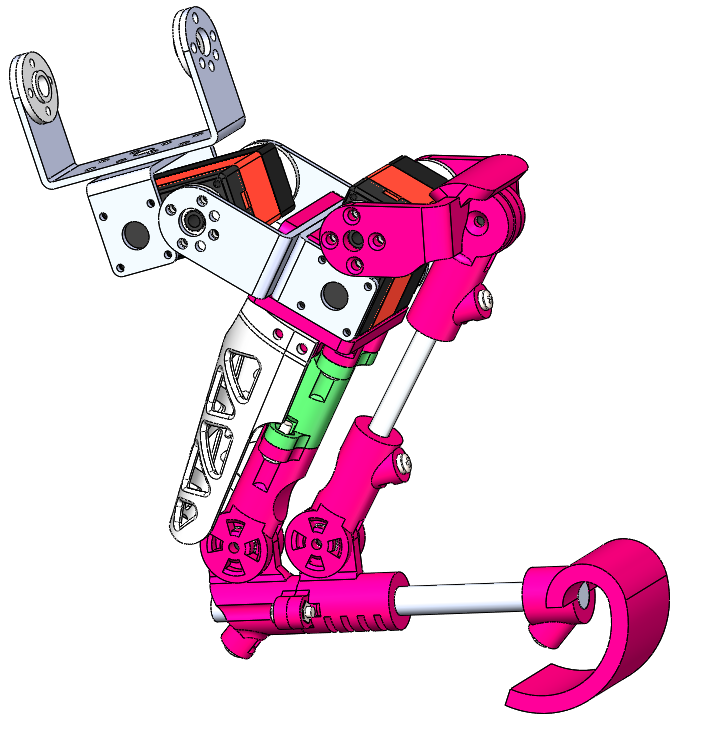
\includegraphics[scale=0.5]{chapter_kinematics/figure2.png}
    \caption{Чертеж конструкции ноги}
    \label{}
\end{figure}

Для упрощения понимания ниже приведена трехмерная кинематическая схема конечности \ref{fig:kin_scheme}.
\begin{figure}[h] %h!
    \centering
    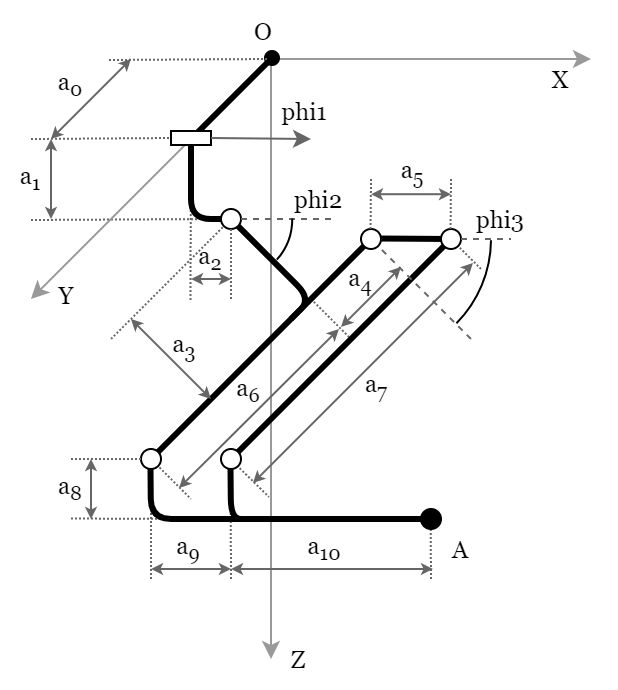
\includegraphics[scale=1.3]{chapter_kinematics/figure1.png}
    \caption{Трехмерная кинематическая схема ноги робота}
    \label{fig:kin_scheme}
\end{figure}

В составе конечности присутствует непрямой кинематический четырехзвенник (три из четырех сторон имеют разные длины). Это усложнило кинематическую задачу, сделало ее менее тривиальной. Как оказалось далее, наличие четырехзвенной передачи сделало невозможным нахождение аналитического решения обратной задачи кинематики. 

На кинематической схеме отмечены величины, численные значения которых приведены ниже:
\begin{align*} % миллиметры вместо метров и знаки препинания
    a_0&=0 \: мм, \\
    a_1&=46.22 \: мм, \\
    a_2&=20 \: мм, \\
    a_3&=44 \: мм, \\
    a_4&=20 \: мм, \\
    a_5&=27 \: мм, \\
    a_6&=87 \: мм, \\
    a_7&=107 \: мм, \\
    a_8&=12.62 \: мм, \\
    a_9&=24.5 \:  мм, \\
    a_{10}&=110  \: мм
\end{align*}

Заметим, что углы $ \varphi_3 $ и $ \varphi_4 $ различаются из-за того что $ a_5 \neq a_9 $. 

Допустимыми диапазонами рабочих углов являются:
\begin{align*}
    \varphi_1&=0 \dots \frac \pi 8, \\
    \varphi_2&=-\frac \pi 2 \dots 0 ,\\
    \varphi_3&=-\frac \pi 4 \dots \frac \pi 4.
\end{align*}

\noindent здесь границы диапазонов выбраны с запасом, чтобы предотвратить соударения составных частей ноги друг с другом. Диапазон для угла $ \varphi_4 $ не указан, поскольку он зависит от $ \varphi_3 $. 

\section{Общее решение четырёхзвенника} \label{sec:pre_direct_kin}

При построении аналитического решения четырехзвенной передачи было важно подобрать функции так, чтобы для рабочих диапазонов углов $ \varphi_1, \varphi_2, \varphi_3 $ не возникало переходов через ноль, или через бесконечно большие числа. Важно избежать использования кусочных функций и условных операторов для упрощения программирования.
Малые диапазоны углов в рассматриваемой конечности облегчают эту задачу.

На рисунке \ref{fig:scheme_four} приведена схема четырехзвенника. Найдем зависимость $ \varphi_4 $ от $ \varphi_3 $. Здесь $ l= a_4 + a_6=a_7 $ введен для упрощения расчётных формул, т.к. две стороны четырехзвенника имеют одну длину.
\begin{figure}[h]
    \centering
    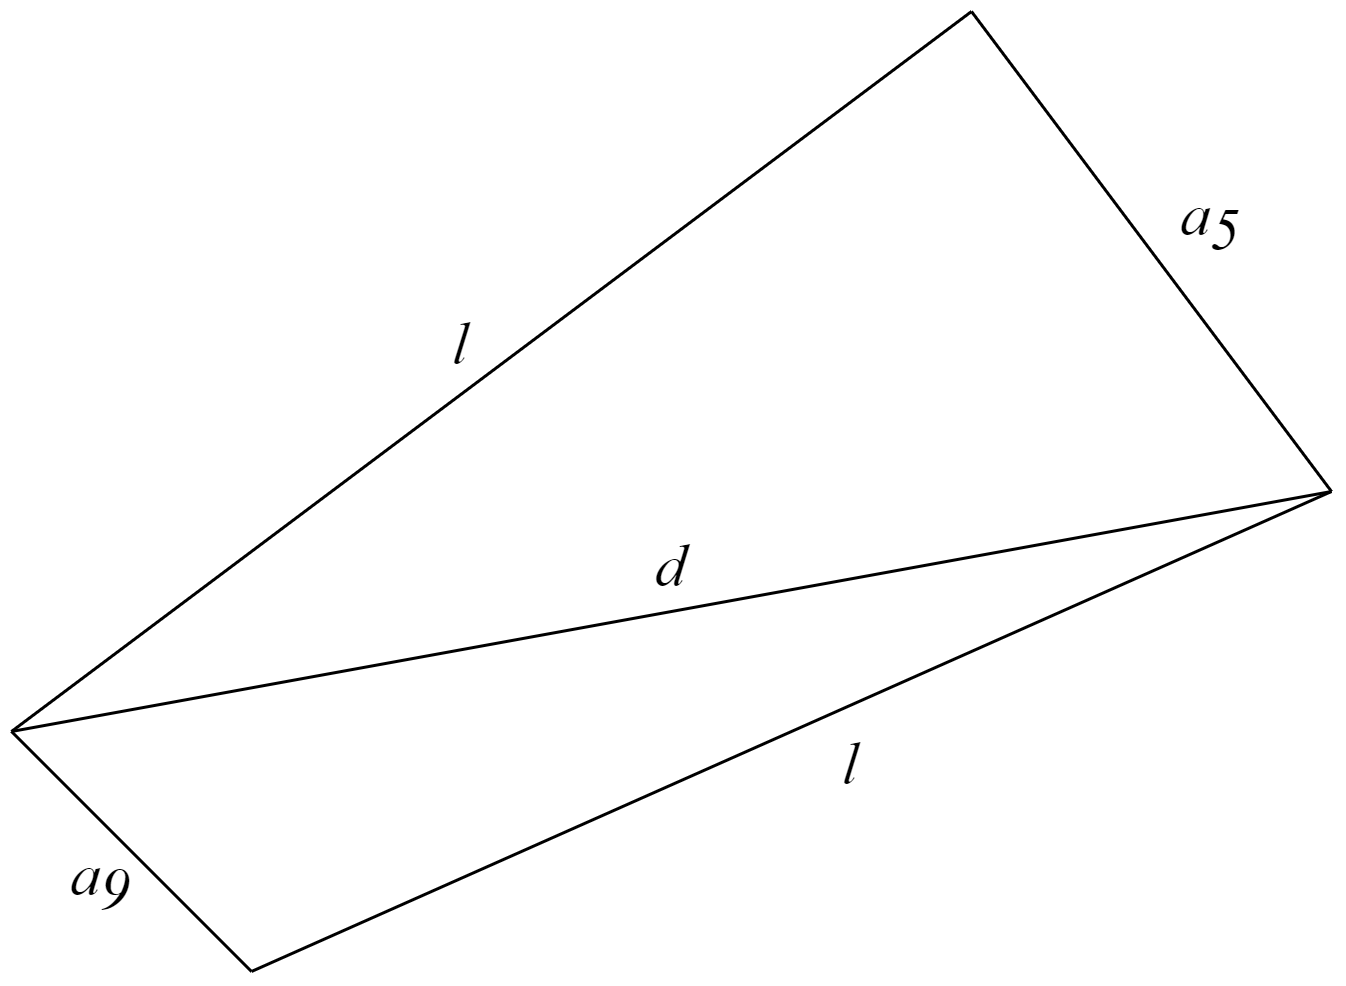
\includegraphics[scale=1]{chapter_kinematics/figure4.png}
    \caption{Четырехзвенник}
    \label{fig:scheme_four}
\end{figure}

Сначала найдем диагональ $d$ по теореме косинусов, для того чтобы выразить противолежащие углы:
\begin{align}
    d = \sqrt{a_5^2 + l^2 - 2a_5 l \cos(\varphi_3)}. \label{eq:kin_1}
\end{align}

\noindent Выразим углы:
\begin{align}
    \gamma &= \text{arcsin}\left(\frac{a_5}{d}\cos \varphi_3\right) \label{eq:gamma}, \\
    \delta &= \text{arccos}\left(\frac{d^2+a_9^2-l^2}{2 a_9 l}\right). \label{eq:delta}
\end{align}

\noindent И искомый угол $ \varphi_4 $ будет находиться следующим образом:
\begin{align}
    \varphi_4 = \pi - \gamma - \delta. \label{eq:phi4_simple}
\end{align}

\noindent Подставим результаты \ref{eq:kin_1}, \ref{eq:gamma}, \ref{eq:delta} в уравнение \ref{eq:phi4_simple} и получим зависимость $ \varphi_4 $ от $ \varphi_3 $:
\begin{multline}
    \varphi_4 = \pi - \text{arcsin}\left(\frac{a_5}{\sqrt{a_5^2 + l^2 - 2a_5 l \cos(\varphi_3)}}\cos \varphi_3\right) - \\ - \text{arccos}\left(\frac{a_5^2 + l^2 - 2a_5 l \cos(\varphi_3)+a_9^2-l^2}{2 a_9 l}\right) .
\end{multline}

\section{Прямая кинематика}\label{sec:direct_kinematics}
Используя найденную в пункте \ref{sec:pre_direct_kin} связь, найдем решение задачи о положении точки $ A $. Трехмерная кинематическая схема приведена на рисунке \ref{fig:kin_scheme}. Зафиксируем сначала первую степень свободы ($ \varphi_1 = 0 $) и найдем координаты точки $ A $ в плоскости, параллельной плоскости $ XZ $:
\begin{multline}
    X_A=a_2+a_3\cos(\varphi_2)+a_6\sin(\varphi_2)-\\-a_8 \cos(\varphi _2+\varphi _4)+(a_9+a_{10}) \sin(\varphi _2+\varphi _4) ,
\end{multline}
\begin{multline} % написать вертикальную черту и phi1=0
    Z_A\Bigr|_{\varphi_1=0} =a_1-a_3 \sin(\varphi _2)+a_6 \cos(\varphi _2)+\\+a_8 \sin(\varphi _2+\varphi _4)+(a_9+a_{10}) \cos(\varphi _2+\varphi _4)
\end{multline}

\noindent Если мы предположим, что $ \varphi_1 = \frac \pi 2 $, тогда конечность будет <<поднята над землей>> в таком положении. Координата $ Z $ точки $ A $ станет равна нулю, координата $ Y $ увеличится. Так как от $ \varphi_1 $ зависят только координаты $Y$ и $Z$, получим следующие уравнения для координат точки $A$:
\begin{multline}
    X_A=a_2+a_3\cos(\varphi_2)+a_6\sin(\varphi_2)-\\-a_8 \cos(\varphi _2+\varphi _4)+(a_9+a_{10}) \sin(\varphi _2+\varphi _4) ,
\end{multline}
\begin{multline}
    Y_A=a_0+\sin(\varphi_1)[a_1-a_3 \sin(\varphi _2)+a_6 \cos(\varphi _2)+\\+a_8 \sin(\varphi _2+\varphi _4)+(a_9+a_{10}) \cos(\varphi _2+\varphi _4)] ,
\end{multline}
\begin{multline}
    Z_A=\cos(\varphi_1)[a_1-a_3 \sin(\varphi _2)+a_6 \cos(\varphi _2)+\\+a_8 \sin(\varphi _2+\varphi _4)+(a_9+a_{10}) \cos(\varphi _2+\varphi _4)].
\end{multline}

\noindent Таким образом, прямая задача кинематики решена.

Получив решение прямой задачи кинематики построим <<рабочую область>> ноги в системе координат связанной с корпусом. Если зафиксировать первую степень свободы, $ \varphi_1 = 0 $, то рабочая область ноги будет лежать в плоскости $ XZ $ (рисунок~\ref{fig:rab_obl}).
\begin{figure}[h]
    \centering
    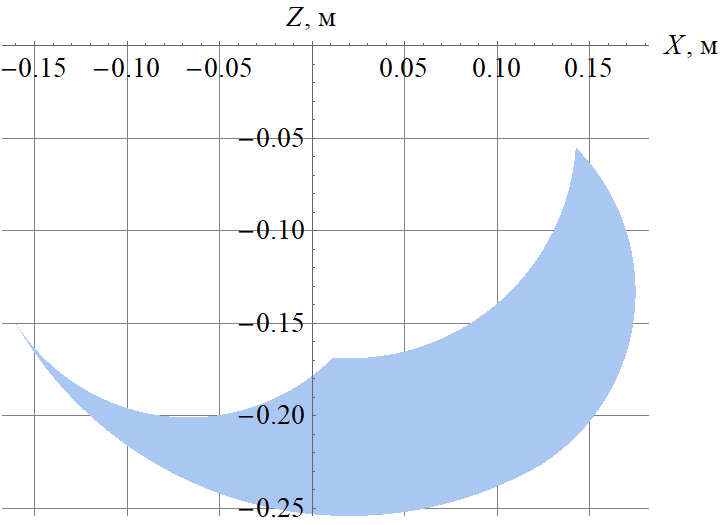
\includegraphics[scale=0.5]{chapter_kinematics/figure3.png}
    \caption{Сечение рабочей области конечности робота}
    \label{fig:rab_obl}
\end{figure}

Следует отметить, что из-за того что $ a_9 < a_5 $, диапазон углов $ \varphi_4 $ получился шире, чем у $ \varphi_3 $. Это наглядно можно продемонстрировать на проекции ноги на плоскость $ XZ $. На рисунке~\ref{fig:leg_model} синей точкой отмечено реальное положение точки $ A $. Красной точкой отмечено положение точки $ A $ в том случае, если бы в четырехзвеннике $ a_5 $ был равен $ a_9 $. В крайних положениях третье звено конечности поворачивается на угол немного больший, чем угол поворота вала сервопривода. C использованием формулы прямой кинематики на рисунке~\ref{fig:leg_model} были изображены предельные положения последнего звена.
\begin{figure}[ht]
    \centering
    % левая картинка
    \begin{subfigure}[b]{0.45\textwidth}    
        \centering
        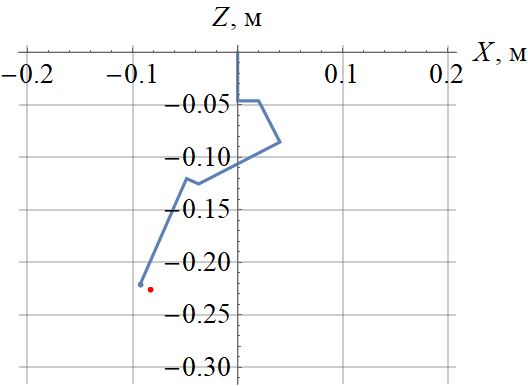
\includegraphics[scale=0.4]{chapter_kinematics/figure5.png}
        \caption{}
    \end{subfigure}
    % правая картинка  
    \begin{subfigure}[b]{0.45\textwidth}
        \centering
        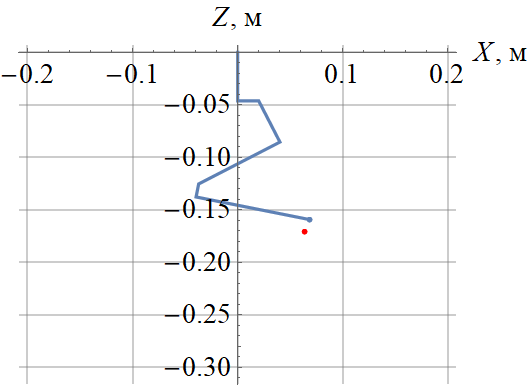
\includegraphics[scale=0.4]{chapter_kinematics/figure6.png}
        \caption{}
    \end{subfigure}
     
    \caption{Проекция ноги на плоскость $ XZ $: \\ (a) третье звено полностью <<разогнуто>>; \\ (б) третье звено полностью <<согнуто>>.}
    \label{fig:leg_model}
\end{figure} % ПОЯСНИТЬ

Так, за счет использования четырехзвенной передачи, увеличена рабочая область конечности. На рисунке \ref{fig:fig7} серая область -- рабочая область при $ a_5 = a_9 $, зеленая область -- расширение рабочей области при $ a_5 > a_9 $.
\begin{figure}[h]
    \centering
    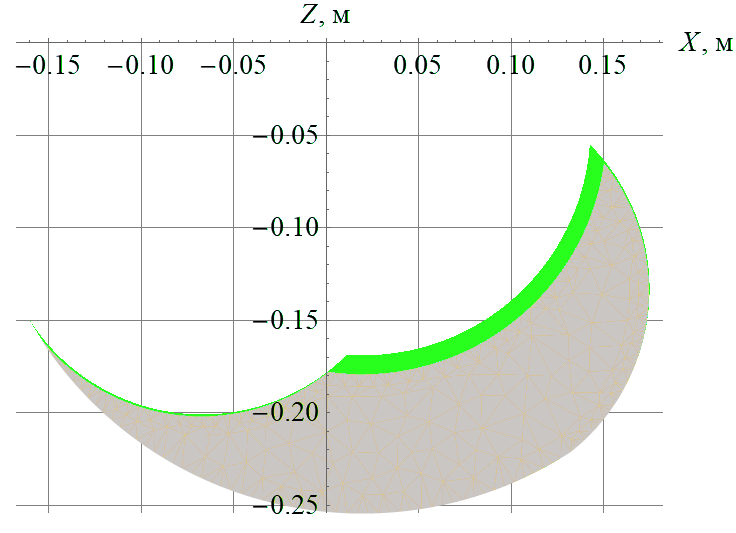
\includegraphics[scale=0.8]{chapter_kinematics/figure8.png}
    \caption{Сравнение рабочих областей}
    \label{fig:fig7}
\end{figure}

\section{Обратная кинематика} \label{sec:inverse_kin}
Как уже упоминалось ранее в пункте \ref{sec:kin_general}, аналитическое решение для задачи обратной представляет большую сложность. Это значит что нужно использовать численные методы решения.

Найдем решение обратной задачи кинематики с помощью метода Ньютона.

Кратко опишем суть метода Ньютона для решения системы нелинейных уравнений. 

Пусть дана система из $ n $ нелинейных уравнений с $ n $ неизвестными:
\[
\left\{ 
\begin{array}{c}
    f_1(x_1, \dots, x_n) = 0, \\
    f_2(x_1, \dots, x_n) = 0, \\
    \vdots \\
    f_i(x_1, \dots, x_n) = 0, \\
\end{array} 
\right.
\]

\noindent где $ f_i(x_1,\dots,x_n): \mathbb{R}^n \rightarrow \mathbb{R}, i=1,\dots, n $ -- нелинейные функции, определенные и непрерывно дифференцируемые в некоторой области $ G \subset \mathbb{R}^n $. Для записи в векторном виде введем величины:
\begin{align*}
    \overline{x} &= [x_1, x_2, \dots x_n]^T, \\
    F(x) &= [f_1(x), f_2(x),\dots,f_n(x)]^T = 0
\end{align*}

Нужно найти такой вектор $ \overline{x}^*=[x_1^*, x_2^*, \dots x_n^*]^T $, чтобы было верно равенство $ F(\overline{x}^*) = 0 $. 

Решение уточняется с помощью итерационной процедуры:
\begin{align*} % 
    x^{(k+1)}=x^{(k)}-J^{-1}(x^{(k)}) \cdot F(x^{(k)}),
\end{align*} % уточнить что такое k

\noindent где $ k=1,2\dots $ -- номер итерации, $ x^{(k)} $ -- $k$-е приближение к корню $ \overline{x}^* $, а $ J $ -- матрица Якоби:
\begin{align*}
    J = \begin{bmatrix}
        \frac{\partial f_1}{\partial x_1} & \dots & \frac{\partial f_1}{\partial x_n} \\
        \vdots & \ddots & \vdots \\
        \frac{\partial f_n}{\partial x_1} & \dots & \frac{\partial f_n}{\partial x_n}
    \end{bmatrix}
\end{align*}

Применительно к задаче, рассматриваемой в данной работе, вектор $ \overline{x} $ является  вектором углов $ \overline{\varphi} = [ \varphi_1, \varphi_2, \varphi_3 ]^T $. Вектор $ F(x) $ -- это правая часть уравнений прямой кинематики.
\begin{equation*}
    F(\overline{\varphi}) = [ X_A(\overline{\varphi}) - X_A^*, Y_A(\overline{\varphi}) - Y_A^*, Z_A(\overline{\varphi}) - Z_A^* ]^T,
\end{equation*}
где $ X_A^*, Y_A^*, Z_A^* $ -- координаты целевого положения точки $A$.

В качестве критерия остановки итераций используется выполнение условия $ \norm{F(\varphi^{(k)}) - F^* } < \varepsilon $, где $\varepsilon $ -- заданная точность позиционировая.

Алгоритм поиска решения обратной задачи представлен ниже. В нём $ \varphi^{(0)} $ -- начальное приближение, $ \varepsilon $ -- точность вычислений, $ i $ -- число итераций (перед выполнением алгоритма устанавливается равным нулю).
\begin{itemize}
    \item[1.] Расчёт Якобиана $$ J = \begin{bmatrix}
        \frac{\partial X_A}{\partial \varphi_1} & 
        \frac{\partial X_A}{\partial \varphi_2} & 
        \frac{\partial X_A}{\partial \varphi_3} \\ \\
        \frac{\partial Y_A}{\partial \varphi_1} & 
        \frac{\partial Y_A}{\partial \varphi_2} & 
        \frac{\partial Y_A}{\partial \varphi_3} \\ \\
        \frac{\partial Z_A}{\partial \varphi_1} & 
        \frac{\partial Z_A}{\partial \varphi_2} & 
        \frac{\partial Z_A}{\partial \varphi_3}
    \end{bmatrix} $$ с использованием формул численного дифференцирования (аналитическая зависимость очень громоздкая).
    \item[2.] Вычисление погрешности: $$ r=F(\varphi^{(k)}). $$
    \item[3.] Вычисление вектора полного шага: $$ p = J^{-1} \cdot r $$ где $ J^{-1} $ -- обратная матрица Якобиана.
    \item[4.] Расчет следующего приближения: $$ \varphi^{(i+1)}=\varphi^{(i)} - p. $$ 
    \item[5.] Если заданная точность не достигнута и не превышен лимит на количество итераций, возвращаемся к пункту 1.
\end{itemize}

\noindent На практике оказалось, что скорость сходимости и сама сходимость сильно зависят от начального приближения. После реализации алгоритма были выявлены две проблемы в его работе:
\begin{itemize}
    \item[1.] Невозможно подобрать такие начальные приближения, при которых бы метод сходился во всем трехмерном пространстве рабочей области.
    \item[2.] В областях, в которых метод сходился в большом удалении от начального приближения, требовалось более 15 итераций для нахождения решения с заданной точностью.
\end{itemize}

\noindent Вторая проблема связана с производительностью вычислителений, которые нужно производить на микрокомпьютере в режиме реального времени. Быстрое решение обратной задачи для любой точки трехмерной рабочей области -- это основное требование которое ставилось в начале разработки системы, поэтому итеративное приближение из предыдущих точек не  подходит в данной ситуации. В следующем пункте приведено решение возникших проблем.

\section{Оптимизация численного решения обратной задачи}

Путем проб и ошибок было решено сохранять в памяти (кэшировать) результаты вычислений прямой кинематики во время запуска программы. Проще говоря, подготовить набор заранее рассчитанных начальных приближений, которые будут использоваться от момента запуска робота до момента завершения работы. Во время решения обратной задачи нужно искать в кэш-таблице ближайшее готовое решение, принимать его за начальное условие текущей задачи и от него досчитывать более точное решение.

В качестве первой реализации две сотни предрассчитанных решений были помещены в кэш-таблицу. Каждая запись в таблице имеет две колонки. В первой колонке помещается вектор координат $ [X_A,Y_A,Z_A] $, во второй колонке вектор соответствующих им углов звеньев $ [\varphi_1, \varphi_2, \varphi_3] $. В момент поиска наилучшего начального приближения для некоторого положения конечности $ [X_A^*,Y_A^*,Z_A^*] $ находится такая запись кэш-таблицы, для которой евклидово расстояние между $ [X_A^*,Y_A^*,Z_A^*] $ и $ [X_A,Y_A,Z_A] $ будет минимально. 

\noindent Простейшая реализация кэширования решений обратной кинематки:

\begin{python}
def cache_inversed_kinematics():
    global cache
    cache = []
    phi1_start, phi1_end = PHI1_RANGE
    phi2_start, phi2_end = PHI2_RANGE
    phi3_start, phi3_end = PHI3_RANGE
    
    for phi1 in np.linspace(phi1_start, phi1_end, num=2):
        for phi2 in np.linspace(phi2_start, phi2_end, num=10):
            for phi3 in np.linspace(phi3_start, phi3_end, num=10):
                angles = [phi1, phi2, phi3]
                cache.append((direct(angles), np.array(angles)))
\end{python}

\noindent Пример реализации поиска решения в кэше:

\begin{python}
def find_nearest_solution(coordinates):
    global cache
    return min(cache, key=lambda di: np.linalg.norm(
        (coordinates - di[0]), 
        ord=2
    ))[1]
\end{python}

Так, получилось решить сразу две проблемы, описанные в пункте \ref{sec:inverse_kin}. Теперь на всей рабочей области обеспечена сходимость алгоритма. Поиск по кэш-таблице гораздо менее затратен, чем итерации метода Ньютона, а после того как найдено <<ближайшее>> решение, метод Ньютона быстро досчитывает ответ в среднем за 2-3 итерации.

\noindent Реализация функции поиска решения обратной задачи выглядит так:
\begin{python}
def inversed(coordinates):
    """ 
    SOLVING THE INVERSE KINEMATICS PROBLEM \n
    Param coordinates is [X, Y, Z] numpy vector, in meters.
    This function uses Newton's numerical method.
    """
    phis = find_nearest_solution(coordinates)
    error = np.ones((3,), dtype=np.float64)

    i = 0
    while np.linalg.norm(error, 2) > 1e-5 and i < 100:
        J = jacobian(phis)
        X = direct(phis)
        error = X - coordinates
        p = np.matmul(np.linalg.pinv(J), error)
        phis = phis - p
        i += 1
    
    return phis
\end{python}

\textbf{Пути для дополнительной оптимизации:}
\begin{itemize}
    \item[1.] Проследить за равномерным распределением кэшированных решений в пространстве рабочей области. В случае равномерного распределения, размер кэша можно сильно уменьшить. Это ускорит поиск по таблице.
    \item[2.] Уменьшать количество кэшированных решений до тех пор пока метод Ньютона продолжает быстро сходиться. Это так же позволит сократить размер кэша и увеличить скорость поиска по нему.
    \item[3.] Найти максимальное значение точности $ \varepsilon $ с учетом ошибок сервоприводов и люфтов конструкции робота. 
\end{itemize}
